\documentclass[landscape, a0]{sciposter}
% Hentet fra http://iacs.epfl.ch/colloqnum06/poster.html
\usepackage[utf8]{inputenc}
\usepackage[T1]{fontenc}
\usepackage[danish]{babel}

\usepackage{amsmath}
\usepackage{amssymb}
\usepackage{multicol}
\usepackage{graphicx}
\usepackage{listings}

\usepackage{epstopdf}
\usepackage{mwe}% for example images

\newcommand{\subcaption}[1]% %1 = text
{\refstepcounter{subfig}%
\par\vskip\abovecaptionskip
\centerline{\textbf{(\alph{subfig})} #1}%
\vskip\belowcaptionskip\par}

% create subfigure environment
\def\subfigure{\let\oldcaption=\caption
\let\caption=\subcaption
\minipage}
\def\endsubfigure{\endminipage
\let\caption=\oldcaption}

\usepackage{xcolor}

\definecolor{dkgreen}{rgb}{0,0.45,0}
\definecolor{gray}{rgb}{0.5,0.5,0.5}
\definecolor{mauve}{rgb}{0.30,0,0.30}

\lstset{frame=tb,
	language=Python,
	aboveskip=4mm,
	belowskip=5mm,
	showstringspaces=false,
	columns=flexible,
	basicstyle={\small\ttfamily},
	numbers=left,
	numberstyle=\footnotesize,
	keywordstyle=\color{dkgreen}\bfseries,
	commentstyle=\color{dkgreen},
	stringstyle=\color{mauve},
	frame=single,
	breaklines=true,
	breakatwhitespace=false,
	tabsize=4,
	xrightmargin=0.50in
}


\usepackage{pgfplots}
\pgfplotsset{
	compat=1.5,
    box plot/.style={
        /pgfplots/.cd,
        black,
        only marks,
        mark=-,
        mark size=1em,
        /pgfplots/error bars/.cd,
        y dir=plus,
        y explicit,
    },
    box plot box/.style={
        /pgfplots/error bars/draw error bar/.code 2 args={%
            \draw  ##1 -- ++(1em,0pt) |- ##2 -- ++(-1em,0pt) |- ##1 -- cycle;
        },
        /pgfplots/table/.cd,
        y index=2,
        y error expr={\thisrowno{3}-\thisrowno{2}},
        /pgfplots/box plot
    },
    box plot top whisker/.style={
        /pgfplots/error bars/draw error bar/.code 2 args={%
            \pgfkeysgetvalue{/pgfplots/error bars/error mark}%
            {\pgfplotserrorbarsmark}%
            \pgfkeysgetvalue{/pgfplots/error bars/error mark options}%
            {\pgfplotserrorbarsmarkopts}%
            \path ##1 -- ##2;
        },
        /pgfplots/table/.cd,
        y index=4,
        y error expr={\thisrowno{2}-\thisrowno{4}},
        /pgfplots/box plot
    },
    box plot bottom whisker/.style={
        /pgfplots/error bars/draw error bar/.code 2 args={%
            \pgfkeysgetvalue{/pgfplots/error bars/error mark}%
            {\pgfplotserrorbarsmark}%
            \pgfkeysgetvalue{/pgfplots/error bars/error mark options}%
            {\pgfplotserrorbarsmarkopts}%
            \path ##1 -- ##2;
        },
        /pgfplots/table/.cd,
        y index=5,
        y error expr={\thisrowno{3}-\thisrowno{5}},
        /pgfplots/box plot
    },
    box plot median/.style={
        /pgfplots/box plot
    }
}


% =========================================================
% ====== Farver og grafik øverst på siden =================
% =========================================================
% Definer farven på baggrunden i overskrifts boksene
\definecolor{BoxCol}{rgb}{0.9,0.9,1}

% Definer farven på tekstn i overskrifts boksene
\definecolor{SectionCol}{rgb}{0,0,0}

% Indsæt logo / billede ved siden af titlen på posteren
\leftlogo[1.6]{fig/julia} 
\rightlogo[1.1]{fig/sdu_segl.pdf} 

% Sæt bredden af de vertikale linier mellem spalterne
\setlength{\columnseprule}{1pt}

% Sæt afstanden mellem to kolonner
%\setlength{\columnsep}{20pt}


% =========================================================
% ====== Informationer om hvem der står bag posteren ======
% =========================================================
% Definer informationer omkring titel, forfattere og 
% organisationen bag.
\title{Who's Julia?}

% Note: only give author names, not institute
\author{Simon Knudsen, Sonni Jensen, Asbjørn Jensen}
 
% insert correct institute name
\institute{Department of Mathematics and Computer Science,\\
	University of Southern Denmark\\}

% Kontakt adresse, kan udelades
%\email{henrik@midtiby.dk}  % shows author email address below institute

%define conference poster is presented at (appears as footer)
\conference{NAT 501 poster session, Juni 2016 SDU Odense}


% =========================================================
% ====== Start på selve indholdet af posteren =============
% =========================================================
\begin{document}

\maketitle

%%% Begin of Multicols-Enviroment
\begin{multicols}{3}


% =========================================================
% ====== Første del =======================================
% =========================================================
\section{Introduction}
Java, C++ and Python are on the top ten of the most used programming languages. There are hundreds of languages, but not minding the hard competition, new languages are still created with the thought of doing better. An example of this is the relatively new programming language Julia, which has been developed with the idea to combine the best features of other languages.\\
\\
The purpose is to find out how well Julia perform compared to some of the standard languages as of 2016. Julia will be compared to Python, Java and C++. Julia draws a lot of inspiration from Python, including syntax and the dynamic type system. Julia shares similarities with Java, mostly behind the scene mechanics, such as garbage collection and compiler optimizations. C++ was chosen since the developers of Julia claim that Julia is as fast as C.

\section{Julia}
Julia is an object-oriented programming language, which has been under development since 2009. First released in 2012 and the newest stable version of Julia is version 0.4.5. The language has been created because the developers wanted a language with all the features they like from other languages. \\
\\
The developers wanted the language to be open source, which means that everybody can read and modify the language. One of the ideas was to make the language as simple, readable and easy to learn as possible. The language is made for high performance and scientific computations while still supporting general purpose programming.

% =========================================================
% ====== Anden del ========================================
% =========================================================
\section{Project Euler problem 116}
\textit{A row of five black square tiles is to have a number of its tiles replaced with coloured tiles from red(length two), green(length three), or blue(length four). If red tiles are chosen there are seven ways. If green tiles are chosen there are three ways. And if blue tiles are chosen there are two ways. Assuming that colours cannot be mixed there are $7+3+2=12$ ways of replacing the black tiles in a row measuring five units in length.}
\begin{figure}[H]
	\centering
	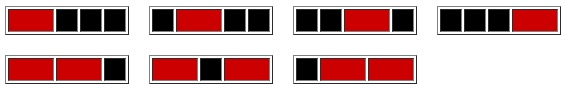
\includegraphics[scale=1.635]{fig/1161.jpg}
	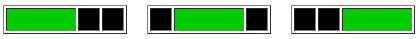
\includegraphics[scale=2.2]{fig/1162.jpg} 
	
\includegraphics[scale=2.2]{fig/1163.jpg} 
\end{figure}
\begin{figure}[H]
	\centering
	\begin{lstlisting}
	function solve(tileSize, squareSize) #m=color block size  n = black box size
		if tileSize > squareSize
			return 0
		end
		solutions = 0
	
		for i = tileSize : squareSize
			solutions += 1
			solutions += solve(tileSize, squareSize-i)
		end
	
		return solutions
	end
	
	function calc(size)
		result = solve(2, size) #Red tiles
		result += solve(3, size) #Green tiles
		result += solve(4, size) #Blue tiles
	
		return result
	end
	\end{lstlisting}
	\caption{Julia implementation}
\end{figure}

\begin{figure}
 \centering
 \hspace*{-0.8in}
 \begin{subfigure}{0.30\textwidth}
		\centering
		\scalebox{.8}{
		\begin{tikzpicture}
			\begin{axis} [
			title=Euler 116 - Julia,
			xlabel={$Input$},
			ylabel={$Time [s]$},
			grid=major,]
				\addplot [box plot median] table {../graphdata/euler116ub-julia-box.dat};
				\addplot [box plot box] table {../graphdata/euler116ub-julia-box.dat};
				\addplot [box plot top whisker] table {../graphdata/euler116ub-julia-box.dat};
				\addplot [box plot bottom whisker] table {../graphdata/euler116ub-julia-box.dat};
				\addplot table {../graphdata/euler116ub-julia.dat};
			\end{axis}
		\end{tikzpicture}
		}
 \end{subfigure}
 \hspace*{0.43in}
 \begin{subfigure}{0.30\textwidth}
		\centering
		\scalebox{.8}{
		\begin{tikzpicture}
			\begin{axis} [
			title=Euler 116 - Python,
			xlabel={$Input$},
			grid=major,]
				\addplot [box plot median] table {../graphdata/euler116ub-python-box.dat};
				\addplot [box plot box] table {../graphdata/euler116ub-python-box.dat};
				\addplot [box plot top whisker] table {../graphdata/euler116ub-python-box.dat};
				\addplot [box plot bottom whisker] table {../graphdata/euler116ub-python-box.dat};
				\addplot table {../graphdata/euler116ub-python.dat};
			\end{axis}
		\end{tikzpicture}
		}
 \end{subfigure}
 \hspace*{.43in}
 \begin{subfigure}{0.30\textwidth}
		\centering
		\scalebox{.8}{
		\begin{tikzpicture}
			\begin{axis} [
			title=Euler 116 - Python excluded,
			xlabel={$Test Input$},
			grid=major,
			legend entries={$Julia$,$Java$,$c++$},
			legend style={at={(1,1)},anchor=north west},
			]
			\addplot table {../graphdata/euler116ub-julia.dat};
			\addplot table {../graphdata/euler116ub-java.dat};
			\addplot table {../graphdata/euler116ub-cpp.dat};
			\end{axis}
		\end{tikzpicture}
		}
 \end{subfigure}%
 
 \hspace*{-0.38in}
 \begin{subfigure}{0.30\textwidth}
		\centering
		\scalebox{1.1}{
		\begin{tikzpicture}
			\begin{axis} [
			title=Euler 116 - Java,
			xlabel={$Input$},
			grid=major,]
				\addplot [box plot median] table {../graphdata/euler116ub-java-box.dat};
				\addplot [box plot box] table {../graphdata/euler116ub-java-box.dat};
				\addplot [box plot top whisker] table {../graphdata/euler116ub-java-box.dat};
				\addplot [box plot bottom whisker] table {../graphdata/euler116ub-java-box.dat};
				\addplot table {../graphdata/euler116ub-java.dat};
			\end{axis}
		\end{tikzpicture}
		}
 \end{subfigure}
 \hspace*{0.08in}
 \begin{subfigure}{0.30\textwidth}
		\centering
		\scalebox{1.1}{
		\begin{tikzpicture}
			\begin{axis} [
			title=Euler 116 - C++,
			xlabel={$Input$},
			grid=major,]
				\addplot [box plot median] table {../graphdata/euler116ub-cpp-box.dat};
				\addplot [box plot box] table {../graphdata/euler116ub-cpp-box.dat};
				\addplot [box plot top whisker] table {../graphdata/euler116ub-cpp-box.dat};
				\addplot [box plot bottom whisker] table {../graphdata/euler116ub-cpp-box.dat};
				\addplot table {../graphdata/euler116ub-cpp.dat};
			\end{axis}
		\end{tikzpicture}
		}
 \end{subfigure}
 \hspace*{.43in}
 \begin{subfigure}{0.30\textwidth}
		\centering
		\scalebox{1.1}{
		\begin{tikzpicture}
			\begin{axis} [
			title=Euler 116,
			xlabel={$Test Input$},
			grid=major,
			legend entries={$Julia$,$Java$,$c++$,$Python$},
			legend style={at={(1,1)},anchor=north west},
			]
			\addplot table {../graphdata/euler116ub-julia.dat};
			\addplot table {../graphdata/euler116ub-java.dat};
			\addplot table {../graphdata/euler116ub-cpp.dat};
			\addplot table {../graphdata/euler116ub-python.dat};
			\end{axis}
		\end{tikzpicture}
		}
 \end{subfigure}%
 \caption{fig}
\end{figure}

% =========================================================
% ====== Afsnit ===========================================
% =========================================================
\section{Results of Project Euler 116}
It is clear that the graphs are exponential increasing. Another thing to notice is that the input is only increasing by one but is still making a huge difference in the run time. One of the reasons is that the problem is solved with recursion, for every extra one bit of space added to the black box a lot more recursive calls will have to be made.\\
\\
The difference in time between the four languages are as expected. Python does not support any form of tail recursion optimization and the result is really slow. Java and Julia on the other hand does a good job at optimizing the recursive calls and is actually faster than C++ - keep in mind that no compiler flags were used in C++, so the default optimization level is used.\\
\\
Julia and Java is close but Java is a bit faster, which is expected because of the fact that Java has been in development much longer than Julia and has a lot more optimization than Julia.

\section{Pros and Cons of Julia}
\begin{list}{}{}
	\item Advantages:
	\item[$\bullet$] Easy to learn and write
	\item[$\bullet$] Compiler optimizations
	\item[$\bullet$] General good performance
	\item[$\bullet$] No memory issues
\end{list}
\begin{list}{}{}
	\item Disadvantages:
	\item[$\bullet$] Compiler optimization breaks in some cases
	\item[$\bullet$] Not very flexible
	\item[$\bullet$] Missing features and bugs / weird behaviors
\end{list}


\begin{thebibliography}{m}

\bibitem{areference}
An Author
{\em A reference}.
A paper.

\bibitem{somepaper}
An Other Author
{\em A reference}.
Some paper.


\end{thebibliography}


\end{multicols}

\end{document}

